\bta{伏安法测电阻}

\begin{enumerate}[leftmargin=0em]
\renewcommand{\labelenumi}{\arabic{enumi}.}
% A(\Alph) a(\alph) I(\Roman) i(\roman) 1(\arabic)
%设定全局标号series=example	%引用全局变量resume=example
%[topsep=-0.3em,parsep=-0.3em,itemsep=-0.3em,partopsep=-0.3em]
%可使用leftmargin调整列表环境左边的空白长度 [leftmargin=0em]
\item
\exwhere{$ 2014 $年理综新课标\lmd{2}卷}
在伏安法测电阻的实验中,待测电阻$ R_x $约为$ 200 \ \Omega $,电压表$ V $的内阻约为$ 2 \ k\Omega $,电流表$ A $的内阻约为$ 10 \ \Omega $,测量电路中电流表的连接方式如图($ a $)或图($ b $)所示,计算结果由$R _ { x } = \frac { U } { I }$计算得出,式中$ U $与 I 分别为电压表和电流表的读数;若将图($ a $)和图($ b $)中电路测得的电阻值分别记为$ R _{x1} $和$ R _{x2} $,则 \tk{$ R_{x1} $} (填“$ R _{x1} $”或“$ R _{x2} $”)更接近待测电阻的真实值,且测量值$ R _{x1} $ \tk{大于} (填“大于”、“等于”或“小于”)真实值,测量值$ R _{x2} $ \tk{小于} (填“大于”、“等于”或“小于”)真实值。
\begin{figure}[h!]
\centering
\includesvg[width=0.43\linewidth]{picture/svg/608}
\end{figure}


\item 
\exwhere{$ 2017 $年浙江选考卷}
小明用电学方法测量电线的长度,首先小明测得电线铜芯的直径为$ 1.00 \ mm $,估计其长度不超过$ 50 \ m $,(已知铜的电阻率为$ 1.75 \times 10^{-8}\ \Omega \cdot m $),现有如下实验器材:
\xctk{
①量程为$ 3V $、内阻约为$ 3 \ k\Omega $的电压表; \qquad ②量程为$ 0.6A $、内阻约为$ 0.1 \ \Omega $的电流表;\\
③阻值为$ 0-2 \ \Omega $的滑动变阻器; \qquad ④内阻可忽略,输出电压为$ 3V $的电源;\\
⑤阻值为$ R_0=4.30 \ \Omega $的定值电阻; \qquad 开关和导线若干。
}

小明采用伏安法测量电线电阻,正确连接电路后,调节滑动变阻器,电流表的示数从$ 0 $开始增加,当示数为$ 0.5A $时,电压表示数如图$ 1 $所示,读数为 \tk{$ 2.50 $} $ V $,根据小明测量的信息,图$ 2 $中$ P $点应该 \tk{接$ b $} (选填“接$ a $”、“接$ b $”、 “接$ c $”或“不接”), $ Q $点应该 \tk{接$ a $ } (选填“接$ a $”、“接$ b $”、“接$ c $”或“不接”),小明测得的电线长度为 \tk{$ 31.4 $} $ m $。
\begin{figure}[h!]
\centering
\includesvg[width=0.53\linewidth]{picture/svg/611}
\end{figure}

\newpage
\item 
\exwhere{$ 2017 $年海南卷}
某同学用伏安法测量待测电阻的阻值。现有器材为:待测电阻$ R $(阻值约为$ 5 $ $ \Omega $),电源(电动势$ 3 $ $ V $),滑动变阻器(阻值范围$ 0 \sim 10 $ $ \Omega $),电流表(量程$ 0.6 $ $ A $,$ 3 $ $ A $),电压表(量程$ 3 $ $ V $,$ 15 $ $ V $),开关,导线若干。实验要求在测量电路中将电流表外接,滑动变阻器起限流作用。回答下列问题:
\begin{enumerate}
\renewcommand{\labelenumi}{\arabic{enumi}.}
% A(\Alph) a(\alph) I(\Roman) i(\roman) 1(\arabic)
%设定全局标号series=example	%引用全局变量resume=example
%[topsep=-0.3em,parsep=-0.3em,itemsep=-0.3em,partopsep=-0.3em]
%可使用leftmargin调整列表环境左边的空白长度 [leftmargin=0em]
\item
按照实验要求在图($ a $)中画出实物连线图。
\begin{figure}[h!]
\centering
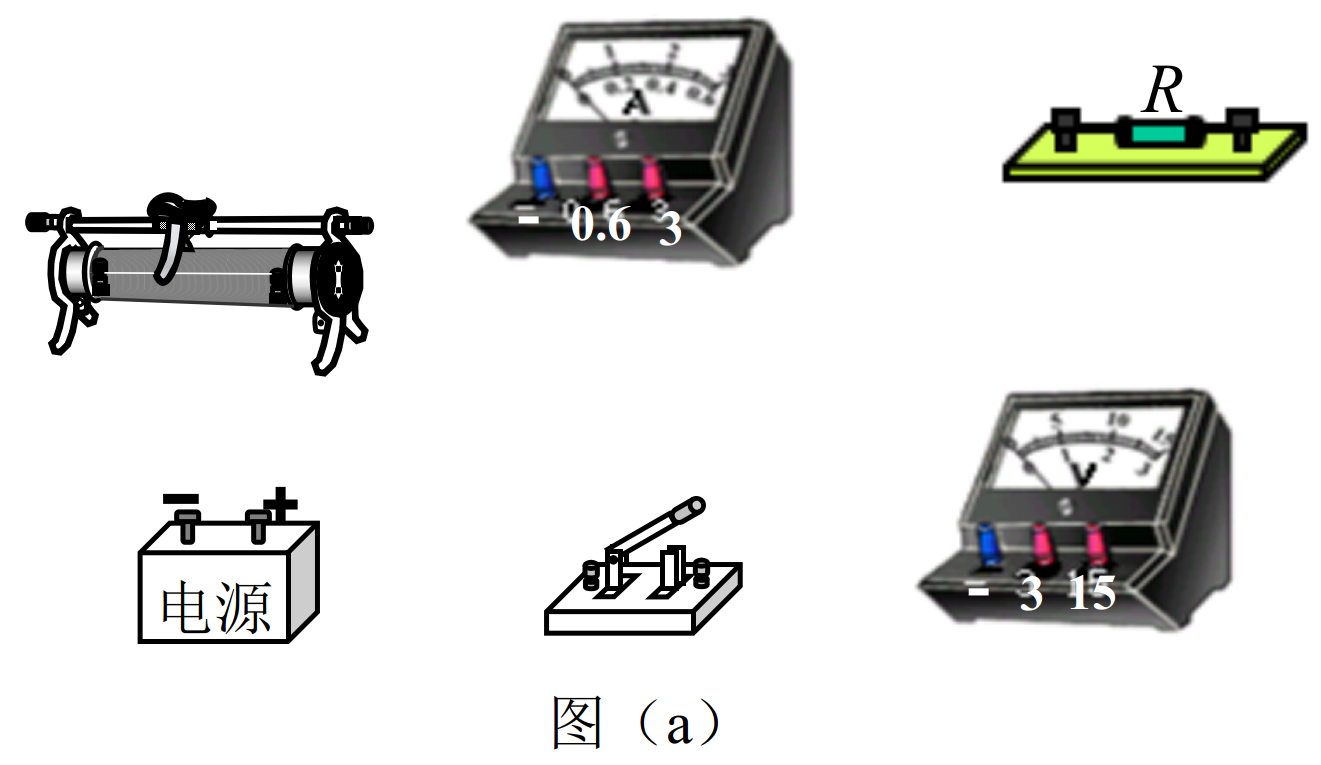
\includegraphics[width=0.7\linewidth]{picture/screenshot006}
\end{figure}


\item 
若已按实验要求接线,闭合开关后移动滑动变阻器的滑片,电压表的示数始终约为$ 3 $ $ V $,电流表的示数始终接近$ 0 $。写出产生这种现象的一个原因: \tk{待测电阻$ R $断路} 。
\item 
在连线正确后,闭合开关。电压表和电流表的示数分别如图($ b $)和图($ c $)所示。由图可知,电压表读数为 \tk{2.20} $ V $,电流表读数为 \tk{0.48} $ A $。由此可得待测电阻的阻值为 \tk{4.58} $ \Omega $(结果保留$ 3 $位有效数字)。
\begin{figure}[h!]
\centering
\includesvg[width=0.48\linewidth]{picture/svg/610}
\end{figure}

\end{enumerate}

\banswer{
实物连线图如右图所示\\
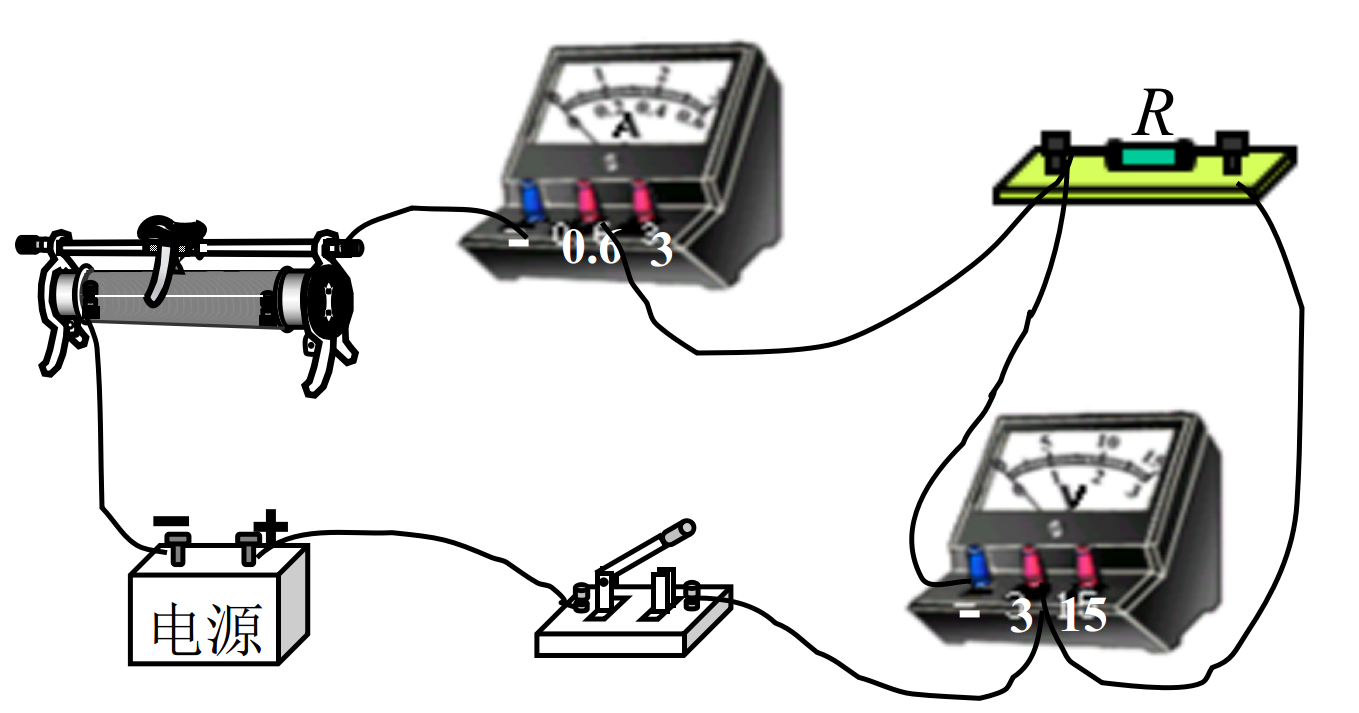
\includegraphics[width=0.7\linewidth]{picture/screenshot007}	
}



\newpage
\item 
\exwhere{$ 2016 $年浙江卷}
某同学用伏安法测量导体的电阻,现有量程为$ 3 $ $ V $、内阻约为$ 3 $ $ k\Omega $的电压表和量程为$ 0..6 $ $ A $、内阻约为$ 0.1 $ $ \Omega $的电流表。采用分压电路接线,图$ 1 $是实物的部分连线图,待测电阻为图$ 2 $中的$ R_{1} $,其阻值约为$ 5 $ $ \Omega $。
\begin{figure}[h!]
\centering
\includesvg[width=0.63\linewidth]{picture/svg/612}
\end{figure}

\begin{enumerate}
\renewcommand{\labelenumi}{\arabic{enumi}.}
% A(\Alph) a(\alph) I(\Roman) i(\roman) 1(\arabic)
%设定全局标号series=example	%引用全局变量resume=example
%[topsep=-0.3em,parsep=-0.3em,itemsep=-0.3em,partopsep=-0.3em]
%可使用leftmargin调整列表环境左边的空白长度 [leftmargin=0em]
\item
测$ R_{1} $阻值的最优连接方式为导线①连接 \tk{a}(填$ a $或$ b $)、导线②连接 \tk{d}(填$ c $或$ d $)。
\item 
正确接线测得实验数据如表,用作图法求得$ R_{1} $的阻值为\tk{$ 4.4\sim 4.7 $ 均可,图见下}$ \Omega $。


\item 
已知图$ 2 $中$ R_{2} $与$ R_{1} $是材料相同、厚度相等、表面为正方形的两导体,$ R_{2} $的边长是$ R_{1} $的$ \frac{1}{10} $,若测$ R_{2} $的阻值,则最优的连线应选 \tk{B}(填选项)。
\fourchoices
{①连接$ a $,②连接$ c $}
{①连接$ a $,②连接$ d $}
{①连接$ b $,②连接$ c $}
{①连接$ b $,②连接$ d $}




\end{enumerate}



\banswer{
(2)作图如下:
\\
\includesvg[width=0.23\linewidth]{picture/svg/613}	
}




\item 
\exwhere{$ 2014 $年物理海南卷}
用伏安法测量一电池的内阻。已知该待测电池的电动势$ E $约为$ 9V $,内阻约数十欧,允许输出的最大电流为$ 50\ mA $,可选用的实验器材有:

\begin{minipage}[h!]{0.7\linewidth}
\vspace{0.3em}
电压表$ V_{1} $(量程$ 5\ V $);电压表$ V_{2} $(量程$ 10\ V $);

电流表$ A_{1} $(量程$ 50\ mA $);电压表$ A_{2} $(量程$ 100\ mA $);

滑动变阻器$ R $(最大电阻$ 300 \ \Omega $);

定值电阻$ R_{1} $(阻值为$ 200 \ \Omega $,额定功率为$ 1/8\ W $);

定值电阻$ R_{2} $(阻值为$ 200 \ \Omega $,额定功率为$ 1\ W $);

开关$ S $;导线若干。
\vspace{0.3em}
\end{minipage}
\hfill
\begin{minipage}[h!]{0.3\linewidth}
\flushright
\vspace{0.3em}
\includesvg[width=0.9\linewidth]{picture/svg/618}
\vspace{0.3em}
\end{minipage}



测量数据如坐标纸上$ U-I $图线所示。
\begin{enumerate}
\renewcommand{\labelenumi}{\arabic{enumi}.}
% A(\Alph) a(\alph) I(\Roman) i(\roman) 1(\arabic)
%设定全局标号series=example	%引用全局变量resume=example
%[topsep=-0.3em,parsep=-0.3em,itemsep=-0.3em,partopsep=-0.3em]
%可使用leftmargin调整列表环境左边的空白长度 [leftmargin=0em]
\item
在答题卡相应的虚线方框内画出合理的电路原理图,并标明所选器材的符号。
\item 
在设计的电路中,选择定值电阻的根据是 \tk{定值电阻在电路中消耗的功率会超过$ 1/8W $, $ R_{2} $的功率满足实验要求} .
\item 
由$ U-I $图线求得待测电池的内阻为 \tk{$ 51.0 $ $ (2 $分。在$ 49.053.0 $范围内的均给分)} $ \Omega $。
\item 
在你设计的电路中,产生系统误差的主要原因是 \tk{忽略了电压表的分流(此答案对应于图$ (a) $) 或:忽略了电流表的分压(此答案对应于图$ (b) $ ) $ (2 $分,其他合理答案也给分)} .





\end{enumerate}

\banswer{
($ 1 $)电路原理图如图$ (a) $所示。$ (5 $分,给出图$ (b) $也给分。原理正确$ 2 $分,仪器选择正确$ 3 $分)\\
\includesvg[width=0.23\linewidth]{picture/svg/619}


}


\newpage

\item
\exwhere{$ 2014 $年理综天津卷}
现要测量一个未知电阻$ R_x $的阻值,除$ R_x $外可用的器材有:

多用电表(仅可使用欧姆挡);

一个电池组$ E $(电动势$ 6V $);

一个滑动变阻器$ R $($ 0 \sim 20 \ \Omega $,额定电流$ 1A $);

两个相同的电流表$ G $(内阻$ R_g=1000 \ \Omega $,满偏电流$ I_g=100\ \mu A $);

两个标准电阻($ R_1=29000 \ \Omega $,$ R_2=0.1 \ \Omega $);

一个电键$ S $、导线若干.

①为了设计电路,先用多用电表的欧姆挡粗测未知电阻,采用“$ \times 10 $”挡,调零后测量该电阻,发现指针偏转非常大,最后几乎紧挨满偏刻度停下来,下列判断的做法正确的是 \tk{AC}(填字母代号).
\fourchoices
{这个电阻很小,估计只有几欧姆}
{这个电阻很大,估计有几千欧姆}
{如需进一步测量可换“$ \times 1 $”挡,调零后测量}
{如需进一步测量可换“$ \times 1k $”挡,调零后测量}

②根据粗测的判断,设计一个测量电路,要求测尽量准确并使电路能耗较小,画出实验电路图,并将各元件字母代码标在该元件的符号旁.

\banswer{
②如右图示\\
\includesvg[width=0.23\linewidth]{picture/svg/614}
}


\item 
\exwhere{$ 2018 $年天津卷}
$ 9 $($ 3 $)某同学用伏安法测定待测电阻$ R_x $的阻值(约为$ 10 $ $ k\Omega $),除了$ R_x $,开关$ S $、导线外,还有下列器材供选用:

A.电压表(量程$ 0 \sim 1 $ $ V $,内阻约为$ 10 $ $ \ k\Omega $)

B.电压表(量程$ 0 \sim 10 $ $ V $,内阻约为$ 100 $ $ \ k\Omega $)

C.电流表($ 0 \sim 1 $ $ m^{A} $内阻约为$ 30 $ $ \Omega $)

D.电流表($ 0 \sim 0.6 $ $ A $,内阻约为$ 0.05 $ $ \Omega $)

$ E $.电源(电动势$ 1.5 $ $ V $,额定电流$ 0.5 $ $ A $,内阻不计)

$ F $.电源(电动势$ 12 $ $ V $,额定电流$ 2 $ $ A $,内阻不计)

$ G $.滑动变阻器$ R_{0} $(阻值范围$ 0 \sim 10 $ $ \Omega $,额定电流$ 2 $ $ A $)

①为使测量尽量准确,电压表选用\tk{B},电流表选用\tk{C},电源选用\tk{F}。(均填器材的字母代号);

②画出测量$ R_x $阻值的实验电路图。

③该同学选择器材、连接电路和操作均正确,从实验原理上看,待测电阻测量值会\tk{大于}其真实值(填“大于”“小于”或“等于”),原因是\tk{电压表的读数大于待测电阻两端实际电压(其他正确表述也可)}。

\banswer{
②实验电路图如答图示\\
\includesvg[width=0.23\linewidth]{picture/svg/615}

}




\item 
\exwhere{$ 2014 $年理综山东卷}
实验室购买了一捆标称长度为$ 100 \ m $的铜导线,某同学想通过实验测定其实际长度。该同学首先测得导线横截面积为$ 1.0\ mm^{2} $,查得铜的电阻率为$1.7 \times 10 ^ { - 8 } \ \Omega \cdot m$,再利用图甲所示电路测出铜导线的电阻$ R_x $,从而确定导线的实际长度。

可供使用的器材有:

\begin{minipage}[h!]{0.7\linewidth}
\vspace{0.3em}
电流表:量程$ 0.6A $,内阻约为$ 0.2 \ \Omega $;

电压表:量程$ 3V $,内阻约$ 9K \ \Omega $;

滑动变阻器$ R_{1} $:最大阻值$ 5 \ \Omega $;

滑动变阻器$ R_{2} $:最大阻值$ 20 \ \Omega $;

定值电阻:$ R_0=3 \ \Omega $;

电源:电动势$ 6V $,内阻可不计;

开关、导线若干。
\vspace{0.3em}
\end{minipage}
\hfill
\begin{minipage}[h!]{0.3\linewidth}
\flushright
\vspace{0.3em}
\includesvg[width=0.9\linewidth]{picture/svg/616}
\vspace{0.3em}
\end{minipage}

回答下列问题:

\begin{enumerate}
\renewcommand{\labelenumi}{\arabic{enumi}.}
% A(\Alph) a(\alph) I(\Roman) i(\roman) 1(\arabic)
%设定全局标号series=example	%引用全局变量resume=example
%[topsep=-0.3em,parsep=-0.3em,itemsep=-0.3em,partopsep=-0.3em]
%可使用leftmargin调整列表环境左边的空白长度 [leftmargin=0em]
\item
实验中滑动变阻器应选\tk{$ R_{2} $}(填“$ R_{1} $”或“$ R_{2} $”),闭合开关$ S $前应将滑片移至\tk{a}端(填“$ a $”或“$ b $”). 
\item 
在实物图(见答题卡)中,已正确连接了部分导线,请根据图甲电路完成剩余部分的连接。
\begin{figure}[h!]
\centering
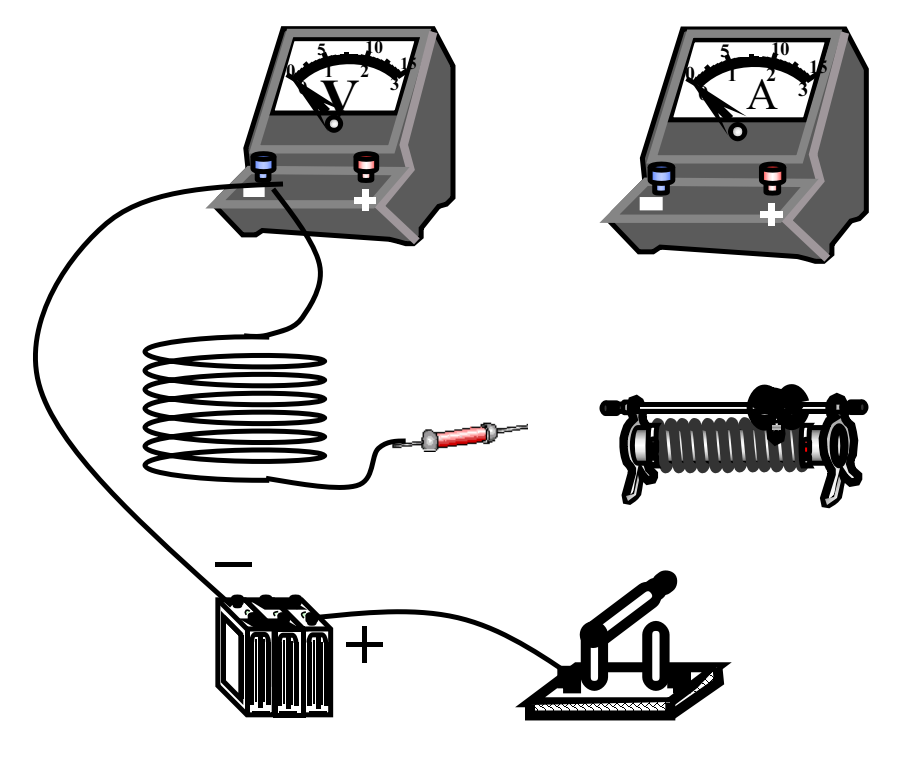
\includegraphics[width=0.5\linewidth]{picture/screenshot008}
\end{figure}


\item 
调节滑动变阻器,当电流表的读数为$ 0.50\ A $时,电压表示数如图乙所示,读数为\tk{$ 2.30 $($ 2.29 $、$ 2.31 $均正确)}$ V $.
\item 
导线实际长度为\tk{$ 94 $($ 93 $、$ 95 $均正确)}$ m $(保留$ 2 $位有效数字).





\end{enumerate}


\banswer{
(2)如图所示\\
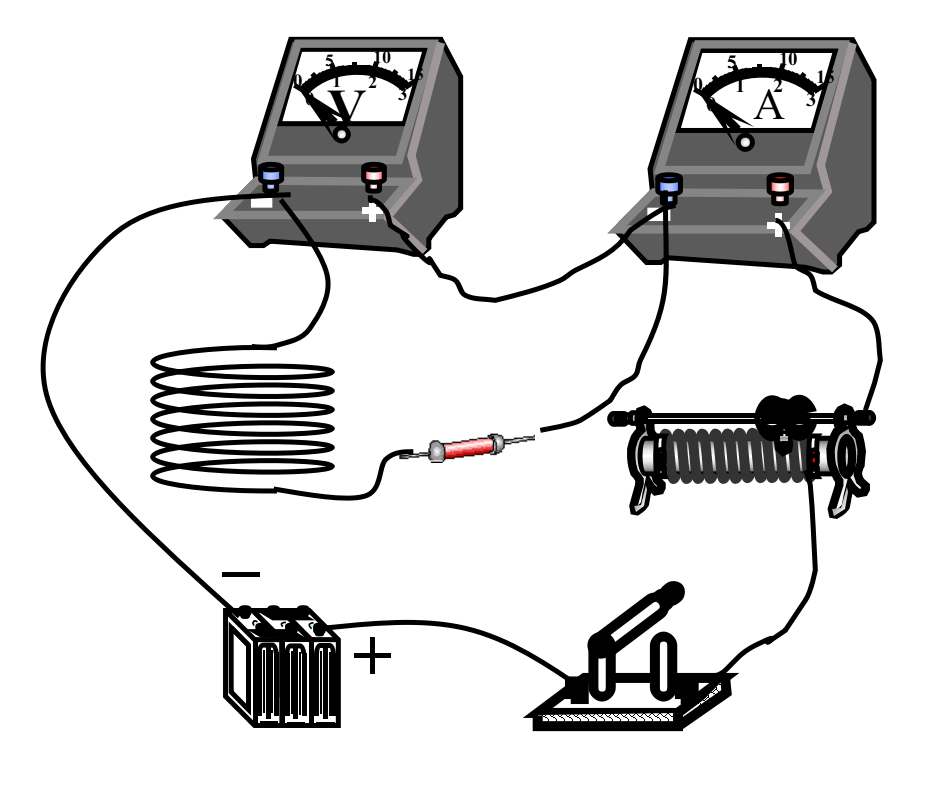
\includegraphics[width=0.5\linewidth]{picture/screenshot009}


}




\newpage
\item 
\exwhere{$ 2014 $年理综浙江卷}
小明对$ 2B $铅笔芯的导电性能感兴趣,于是用伏安法测量其电阻值。
\begin{figure}[h!]
\centering
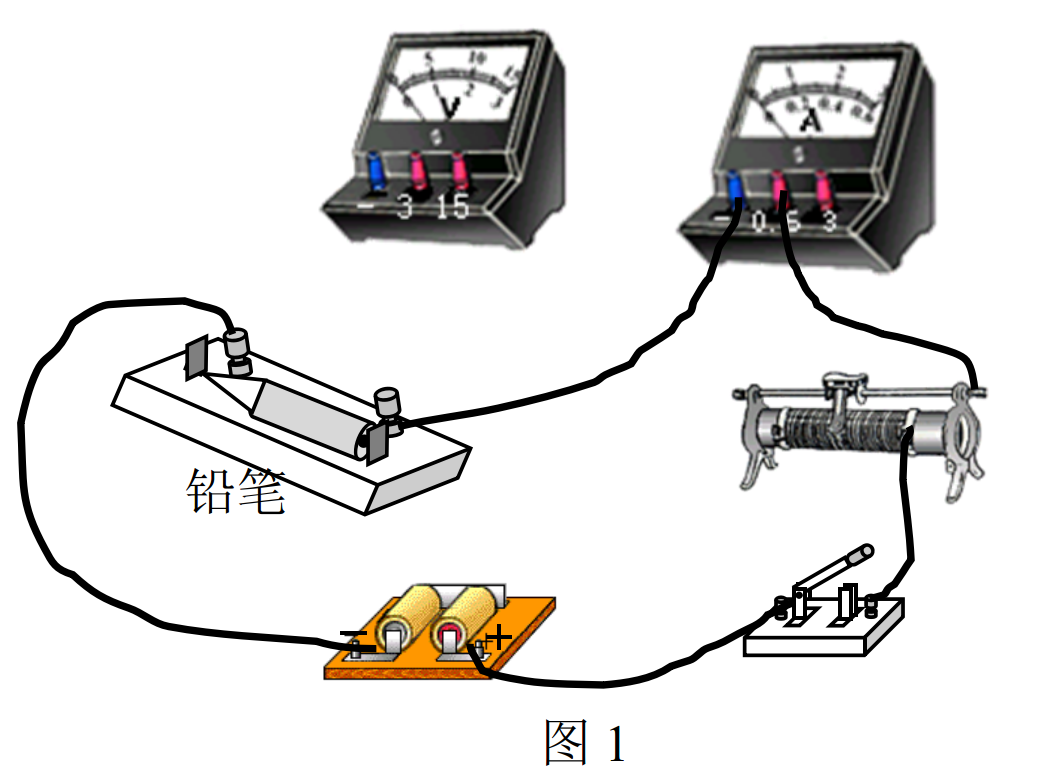
\includegraphics[width=0.45\linewidth]{picture/screenshot010}
\includesvg[width=0.4\linewidth]{picture/svg/620}

\end{figure}

\begin{enumerate}
\renewcommand{\labelenumi}{\arabic{enumi}.}
% A(\Alph) a(\alph) I(\Roman) i(\roman) 1(\arabic)
%设定全局标号series=example	%引用全局变量resume=example
%[topsep=-0.3em,parsep=-0.3em,itemsep=-0.3em,partopsep=-0.3em]
%可使用leftmargin调整列表环境左边的空白长度 [leftmargin=0em]
\item
图$ 1 $是部分连接好的实物电路图,请用电流表外接法完成接线并在图$ 1 $中画出。
\item 
小明用电流表内接法和外接法分别测量了一段$ 2B $铅笔芯的伏安特性,并将得到的电流、电压数据描到$ U-I $图上,如图$ 2 $所示。在图中,由电流表外接法得到的数据点是用 \tk{$ \times $}(填“$ \circ $”或“$ \times $”)表示的。
\item 
请你选择一组数据点,在图$ 2 $上用作图法作图,并求出这段铅笔芯的电阻为\tk{用“$ \times $”数据点连直线,$ R=(1.1 \sim 1.3) \ \Omega $;用“$ \circ $”数据点连直线,同理得$ R=(1.5 \sim 1.7) \ \Omega $}$ \Omega $。



\end{enumerate}


\banswer{
答题图:\\
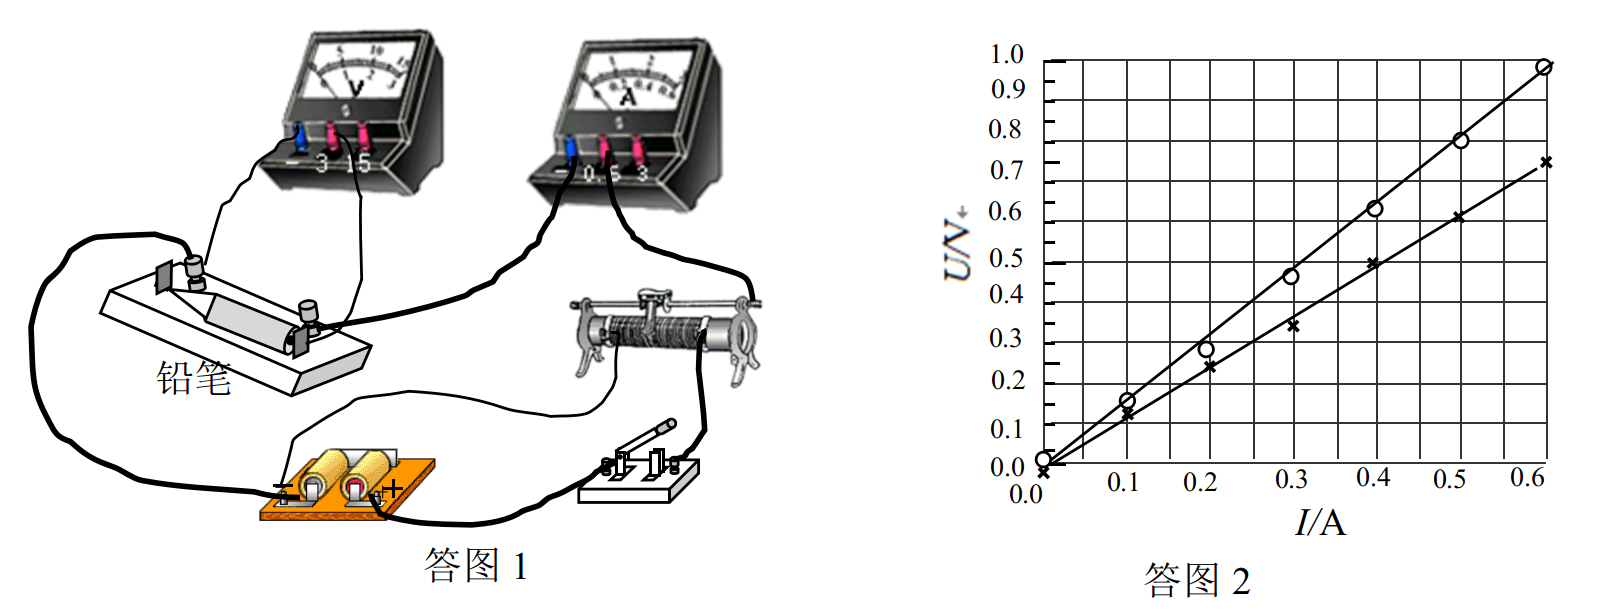
\includegraphics[width=0.8\linewidth]{picture/screenshot011}


}




\item 
\exwhere{$ 2011 $年理综天津卷}
某同学测量阻值约为$ 25k \ \Omega $的电阻$ R_x $ ,现备有下列器材:

A. 电流表(量程$ 100 \mu A $,内阻约$ 2k \ \Omega $);

B. 电流表(量程$ 500 \mu A $,内阻约$ 300 \ \Omega $);

C. 电压表(量程$ 15V $,内阻约$ 100k \ \Omega $);

D. 电压表(量程$ 50V $,内阻约$ 500k \ \Omega $);

$ E $. 直流电源($ 20V $,允许最大电流$ 1A $);

$ F $. 滑动变阻器(最大阻值$ 1k \ \Omega $,额定功率$ 1W $);

$ G $. 电键和导线若干。

电流表应选\tk{B}.电压表应选\tk{C}.(填字母代号)

该同学正确选择仪器后连接了以下电路,为保证实验顺利进行,并使测量误差尽量减小,实验前请你检查该电路,指出电路在接线上存在的问题:

\begin{minipage}[h!]{0.6\linewidth}
\vspace{0.3em}
① \hfullline ;

② \hfullline 。
\vspace{0.3em}
\end{minipage}
\hfill
\begin{minipage}[h!]{0.4\linewidth}
\flushright
\vspace{0.3em}
\includesvg[width=0.94\linewidth]{picture/svg/621}
\vspace{0.3em}
\end{minipage}


\newpage
\item 
\exwhere{$ 2013 $年北京卷}
某同学通过实验测定一个阻值约为$ 5 \ \Omega $的电阻$ R_x $的阻值。

\begin{enumerate}
\renewcommand{\labelenumi}{\arabic{enumi}.}
% A(\Alph) a(\alph) I(\Roman) i(\roman) 1(\arabic)
%设定全局标号series=example	%引用全局变量resume=example
%[topsep=-0.3em,parsep=-0.3em,itemsep=-0.3em,partopsep=-0.3em]
%可使用leftmargin调整列表环境左边的空白长度 [leftmargin=0em]
\item
现有电源($ 4V $,内阻可不计)、滑动变阻器($ 0 \sim 50 \ \Omega $,额定电流$ 2A $),开关和导线若干,以及下列电表:

A.电流表($ 0 \sim 3A $,内阻约$ 0.025 \ \Omega $)

B.电流表($ 0 \sim 0.6A $,内阻约$ 0.125 \ \Omega $)

C.电压表($ 0 \sim 3V $,内阻约$ 3 \ k\Omega $)

D.电压表($ 0 \sim 15V $,内阻约$ 15 \ k\Omega $)

为减小测量误差,在实验中,电流表应选用\tk{B},电压表应选用\tk{C}(选填器材前的字母);实验电路应采用图$ 1 $中的\tk{甲}(选填“甲”或“乙”)。
\begin{figure}[h!]
\centering
\includesvg[width=0.53\linewidth]{picture/svg/622}
\end{figure}

\item 
图$ 2 $是测量$ R_x $的实验器材实物图,图中已连接了部分导线。请请根据在(1)问中所选的电路图,补充完成图$ 2 $中实物间的连线。
\begin{figure}[h!]
\centering
\includesvg[width=0.53\linewidth]{picture/svg/623}
\end{figure}


\item 
接通开关,改变滑动变阻器滑片$ P $的位置,并记录对应的电流表示数 \lmd{1} 、电压表示数$ U $。某次电表示数如图$ 3 $所示,可得该电阻的测量值$R _ { x } = \frac { U } { I } = $ \tk{5.2} $ \Omega $(保留两位有效数字)。
\begin{figure}[h!]
\centering
\includesvg[width=0.43\linewidth]{picture/svg/625}
\end{figure}

\item 
若在($ 1 $)问中选用甲电路,产生误差的主要原因是\tk{B};若在($ 1 $)问中选用乙电路,产生误差的主要原因是 \tk{D} 。(选填选项前的字母)
\fourchoices
{电流表测量值小于流经$ Rx $的电流值}
{电流表测量值大于流经$ Rx $的电流值}
{电压表测量值小于$ Rx $两端的电压值}
{电压表测量值大于$ Rx $两端的电压值}

\item 
在不损坏电表的前提下,将滑动变阻器滑片$ P $从一端滑向另一端,随滑片$ P $移动距离$ x $的增加,被测电阻$ R_x $两端的电压$ U $也随之增加,下列反映$ U-x $关系的示意图中正确的是\tk{A}。
\begin{figure}[h!]
\centering
\includesvg[width=0.63\linewidth]{picture/svg/624}
\end{figure}




\end{enumerate}



\banswer{
 $ (2) $如答图$ 1 $所示:\\
\includesvg[width=0.23\linewidth]{picture/svg/626}
 
}





\newpage
\item 
\exwhere{$ 2013 $年重庆卷}
某同学对有故障的电热毯进行探究。图$ 1 $是电热毯的电路示意图,其中电热线和导线通过金属接线片连接。图$ 2 $为测试电路实物图,$ A $、$ B $为测试表笔,电压表内阻很大,可视为理想电表。
\begin{figure}[h!]
\centering
\includesvg[width=0.73\linewidth]{picture/svg/627}
\end{figure}

①请在答题卡虚线框内画出与图$ 2 $对应的电路图。

②断开$ K_{1} $,用上述测试电路在$ 1 $和$ 1 ^{\prime} $之间检测得知电热线无故障,然后测得电热线的$ U-I $曲线如图$ 3 $所示。已知电热线材料的电阻率为$ 2.8 \times 10^{-7 }\ \Omega \cdot m $,电热线的直径为$ 0.200 \ mm $。可求得此电热线的电阻为 \tk{$ 0.58 $ ($ 0.57 $到$ 0.59 $均可)} $ k \Omega $,总长度为 \tk{$ 65 $($ 64 $到$ 66 $均可)} $ m $。(结果均保留两位有效数字)
\begin{figure}[h!]
\centering
\includesvg[width=0.33\linewidth]{picture/svg/628}
\end{figure}


③为了进一步检查故障,该同学闭合开关$ K_{1} $和$ K_{2} $,用表笔$ A $和$ B $分别对图$ 1 $中所示的各点进行测试,部分测试结果如下表所示。由此测试结果可判断出电路有断路,位置在 \tk{$ 1 ^{\prime} $ 和$ 2 ^{\prime} $} 之间(在“$ 1 $和$ 2 $”、“$ 1 ^{\prime} $ 和$ 2 ^{\prime} $”、“$ 2 $和$ 3 $”、“$ 2 ^{\prime} $ 和$ 3 ^{\prime} $”中选填一项)。




\begin{table}[h!]
\centering 
\begin{tabular}{|c|c|c|c|c|c|c|}
\hline 
\multicolumn{2}{|c|}{测试点} &3和$ 3 ^{\prime} $ & 1和$ 1 ^{\prime} $ & 1和3 & 1和$ 2 ^{\prime} $ &$ 2 ^{\prime} $ 和$ 3 ^{\prime} $ \\
\hline
\multirow{2}{4em}{电表指针有无偏转} & 电压表 & 有 & 有 & 无 & 有 & 无
 \\
\hline
& 电流表 & 无 & 有 & 有 & 无 & 有\\ 
\hline 
\end{tabular}
\end{table} 

\banswer{
①电路图如图示\\
\includesvg[width=0.23\linewidth]{picture/svg/629}


}



\newpage
\item
\exwhere{$ 2015 $年理综四川卷}
用实验测一电池的内阻$ r $和一待测电阻的阻值$ R_x $。已知电池的电动势约$ 6V $,电池内阻和待测电阻阻值都为数十欧。可选用的实验器材有:

电流表$ A_{1} $(量程$ 0 $ – $ 30mA) $;

电流表$ A_{2} $(量程$ 0 $ – $ 100mA) $;

电压表$ V $(量程$ 0 $ – $ 6V) $;

滑动变阻器$ R_{1} $(阻值$ 0 $ –$ 5 \ \Omega ) $;

滑动变阻器$ R_{2} $(阻值$ 0 $ –$ 300 \ \Omega ) $;

开关$ S $一个,导线若干条。
\begin{figure}[h!]
\centering
\includesvg[width=0.33\linewidth]{picture/svg/630} \qquad 
\includesvg[width=0.43\linewidth]{picture/svg/631}
\end{figure}

某同学的实验过程如下:

$ \lmd{1} $.设计如图$ 3 $所示的电路图,正确连接电路。

$ \lmd{2} $.将$ R $的阻值调到最大,闭合开关,逐次调小$ R $的阻值,测出多组$ U $和 \lmd{1} 的值,并记录。以$ U $为纵轴, \lmd{1} 为横轴,得到如图$ 4 $所示的图线。

$ \lmd{3} $.断开开关,将$ Rx $改接在$ B $、$ C $之间,$ A $与$ B $直接相连,其他部分保持不变。重复$ \lmd{2} $的步骤,得到另一条$ U $— \lmd{1} 图线,图线与横轴 \lmd{1} 的交点坐标为($ I_{0} $,$ 0 $),与纵轴$ U $的交点坐标为($ 0 $,$ U_{0} $)。回答下列问题:

①电流表应选用 \tk{$ A_{2} $} ,滑动变阻器应选用 \tk{$ R_{2} $} ; 

②由图$ 4 $的图线,得电源内阻$ r= $ \tk{25} $ \Omega $ ;

③用$ I_{0} $、$ U_{0} $和$ r $表示待测电阻的关系式$ R_x= $ \tk{$\frac { U _ { 0 } } { I _ { 0 } } - r$} ,代入数值可得$ R_x $;

④若电表为理想电表, $ Rx $接在$ B $、$ C $之间与接在$ A $、$ B $之间,滑动变阻器滑片都从最大阻值位置调到某同一位置,两种情况相比,电流表示数变化范围 \tk{相同} ,电压表示数变化范围 \tk{相同}。(选填”相同”或”不同”)




\end{enumerate}

